
\section{ Example}

\noindent In the following example, we use 5 users (i.e., Alice, Bob, Charlie, David and Elizabeth) to show the process of ACP. We should notice that David trusts Charlie (Charlie does not trust David), Elizabeth trusts David (David does not trust Elizabeth). Users do not trust others except the above two pairs. The parameters are shown in Table \ref{table:ACPExampleParameters}.

\begin{table} [hbtp]
\caption{Example Parameters}
\label{table:ACPExampleParameters}
\centering
\tabulinesep=2mm
\begin{tabu}{|c|c|} \hline 
%\begin{tabular}{|c|l|} \hline 
Parameters & Explanation \\ \hline 
${k}$ & 3 \\ \hline 
${m}$ & 1 \\ \hline 
${Seg}$ & 2 \\ \hline 
${GP}$ & 10 minutes \\ \hline 
${AT}$ & 80 minutes \\ \hline 
${\tau}$ & 80 minutes (equal to ${AT}$) \\ \hline 
%\end{tabular}
\end{tabu}
\end{table}

We abstract the event that users encounter each other in Table \ref{table:ACPExampleEvent}. Let $t_i$ denote the $i^{th}$ minute. The table lists the time when two users encounter each other. For example, Charlie and Elizabeth encounter each other at the third minute ($t_3$). After two users meet, they separate in one minute. 

\begin{table} [hbtp]
\caption{Example Event}
\label{table:ACPExampleEvent}
\centering
\tabulinesep=2mm
\begin{tabu}{|c|c|c|} \hline 
%\begin{tabular}{|c|l|} \hline 
User 1 & User 2 & Time \\ \hline 
Elizabeth & Bob & $t_1$ \\ \hline 
Bob & Charlie & $t_2$ \\ \hline 
Charlie & Elizabeth & $t_3$ \\ \hline 
Elizabeth & Alice & $t_4$ \\ \hline 
Bob & Charlie & $t_5$ \\ \hline 
Alice & Charlie & $t_6$ \\ \hline 
Charlie & David & $t_7$ \\ \hline 
David & Elizabeth & $t_8$ \\ \hline 
%\end{tabular}
\end{tabu}
\end{table}

We assume that these users do not encounter any user for a long time, so that they each has 8 ($=\frac{80min}{10min}$) ACs generated by themselves. We also assume that no AC expires in our 8-minutes example. Since the parameter \textit{Seg} is equal to 2, each user has 2 \textit{Distributing} AC Lists (\textit{DL}s). The initial state of our example is shown in Table \ref{table:ACPExampleInitialState}. To make the example simple and clear, we do not place ACs in \textit{DL}s randomly, ACs are always placed in the DL alternately. For example, if we put the first AC in \textit{DL}1, then the second AC must be in the \textit{DL}2. Users also obey the rule when they receive ACs from other users.

\begin{table} [hbtp]
\caption{Example Initial State}
\label{table:ACPExampleInitialState}
\centering
\tabulinesep=2mm
\begin{tabu}{|c|l|l|l|} \hline 
User Identity & \textit{DL}1 & \textit{DL}2 & \textit{RL} \\ \hline 
Alice (A) & ${\mathrm{AC}}^{\mathrm{1}\left[0\right]}_{\mathrm{A}},{\mathrm{AC}}^{\mathrm{3}\left[0\right]}_{\mathrm{A}},{\mathrm{AC}}^{\mathrm{5}\left[0\right]}_{\mathrm{A}},{\mathrm{AC}}^{\mathrm{7}\left[0\right]}_{\mathrm{A}}$ & ${\mathrm{AC}}^{\mathrm{2}\left[0\right]}_{\mathrm{A}},{\mathrm{AC}}^{\mathrm{4}\left[0\right]}_{\mathrm{A}},{\mathrm{AC}}^{\mathrm{6}\left[0\right]}_{\mathrm{A}},{\mathrm{AC}}^{\mathrm{8}\left[0\right]}_{\mathrm{A}}$ & $\mathrm{\emptyset }$ \\ \hline 
Bob (B) & ${\mathrm{AC}}^{\mathrm{1}\left[0\right]}_{\mathrm{B}},{\mathrm{AC}}^{\mathrm{3}\left[0\right]}_{\mathrm{B}},{\mathrm{AC}}^{\mathrm{5}\left[0\right]}_{\mathrm{B}},{\mathrm{AC}}^{\mathrm{7}\left[0\right]}_{\mathrm{B}}$ & ${\mathrm{AC}}^{\mathrm{2}\left[0\right]}_{\mathrm{B}},{\mathrm{AC}}^{\mathrm{4}\left[0\right]}_{\mathrm{B}},{\mathrm{AC}}^{\mathrm{6}\left[0\right]}_{\mathrm{B}},{\mathrm{AC}}^{\mathrm{8}\left[0\right]}_{\mathrm{B}}$ & $\mathrm{\emptyset }$ \\ \hline 
Charlie (C) & ${\mathrm{AC}}^{\mathrm{1}\left[0\right]}_{\mathrm{C}},{\mathrm{AC}}^{\mathrm{3}\left[0\right]}_{\mathrm{C}},{\mathrm{AC}}^{\mathrm{5}\left[0\right]}_{\mathrm{C}},{\mathrm{AC}}^{\mathrm{7}\left[0\right]}_{\mathrm{C}}$ & ${\mathrm{AC}}^{\mathrm{2}\left[0\right]}_{\mathrm{C}},{\mathrm{AC}}^{\mathrm{4}\left[0\right]}_{\mathrm{C}},{\mathrm{AC}}^{\mathrm{6}\left[0\right]}_{\mathrm{C}},{\mathrm{AC}}^{\mathrm{8}\left[0\right]}_{\mathrm{C}}$ & $\mathrm{\emptyset }$ \\ \hline 
David (D) & ${\mathrm{AC}}^{\mathrm{1}\left[0\right]}_{\mathrm{D}},{\mathrm{AC}}^{\mathrm{3}\left[0\right]}_{\mathrm{D}},{\mathrm{AC}}^{\mathrm{5}\left[0\right]}_{\mathrm{D}},{\mathrm{AC}}^{\mathrm{7}\left[0\right]}_{\mathrm{D}}$ & ${\mathrm{AC}}^{\mathrm{2}\left[0\right]}_{\mathrm{D}},{\mathrm{AC}}^{\mathrm{4}\left[0\right]}_{\mathrm{D}},{\mathrm{AC}}^{\mathrm{6}\left[0\right]}_{\mathrm{D}},{\mathrm{AC}}^{\mathrm{8}\left[0\right]}_{\mathrm{D}}$ & $\mathrm{\emptyset }$ \\ \hline 
Elizabeth (E) & ${\mathrm{AC}}^{\mathrm{1}\left[0\right]}_{\mathrm{E}},{\mathrm{AC}}^{\mathrm{3}\left[0\right]}_{\mathrm{E}},{\mathrm{AC}}^{\mathrm{5}\left[0\right]}_{\mathrm{E}},{\mathrm{AC}}^{\mathrm{7}\left[0\right]}_{\mathrm{E}}$ & ${\mathrm{AC}}^{\mathrm{2}\left[0\right]}_{\mathrm{E}},{\mathrm{AC}}^{\mathrm{4}\left[0\right]}_{\mathrm{E}},{\mathrm{AC}}^{\mathrm{6}\left[0\right]}_{\mathrm{E}},{\mathrm{AC}}^{\mathrm{8}\left[0\right]}_{\mathrm{E}}$ & $\mathrm{\emptyset }$ \\ \hline 
\end{tabu}
\end{table}

The explanation of symbols used in table are shown in the former Table \ref{table:ACPSymbols}. To make the symbol clear, we add the \textit{EQL} of the AC on the superscript. For example, if the \textit{EQL} of ${AC}^1_{A,X}$ is equal to 2, it is marked as ${AC}^{1\left[2\right]}_{A,X}$.


\subsection{ Exchanging Appointment Cards}

\noindent To make it easier, users do not pick \textit{DL}s randomly as we described in the previous sections when they exchange ACs. Instead, If we say that $U_x$ encounters $U_y$, $U_x$ always picks his \textit{DL}1 and $U_y$ always picks his \textit{DL}2. 

The tables in current section show the entire \textit{distributing}-AC Lists (i.e., \textit{DL}1 and \textit{DL}2) and entire \textit{relay-table}s (\textit{RL}s) of each user. We use the initial letter to denote each user in symbols. For example, D denotes David. The structure of the AC-list tables is shown in Table \ref{table:ACPXYACLists}.

\begin{table} [H]
\caption{User X and Y's AC Lists}
\label{table:ACPXYACLists}
\centering
\tabulinesep=2mm
\begin{tabu}{|c|c|c|l|} \hline 
\multirow{6}*{X} & \multirow{2}*{\textit{DL}1} & Before & X's \textit{distributing}-AC list 1 before their exchange. \\ \cline{3-4}
 &  & After & X's \textit{distributing}-AC list 1 after their exchange. \\ \cline{2-4} 
 & \multirow{2}*{\textit{DL}2} & Before & X's \textit{distributing}-AC list 2 before their exchange. \\ \cline{3-4} 
 &  & After & X's \textit{distributing}-AC list 2 after their exchange. \\ \cline{2-4} 
 &\multirow{2}*{ \textit{RL}} & Before & X's \textit{ready}-AC list before their exchange. \\ \cline{3-4} 
 &  & After & X's \textit{ready}-AC list after their exchange. \\ \hline 
\multirow{6}*{Y} & \multirow{2}*{\textit{DL}1} & Before & Y's \textit{distributing}-AC list 1 before their exchange. \\ \cline{3-4} 
 &  & After & Y's \textit{distributing}-AC list 1 after their exchange. \\ \cline{2-4} 
 & \multirow{2}*{\textit{DL}2} & Before & Y's \textit{distributing}-AC list 2 before their exchange. \\ \cline{3-4} 
 &  & After & Y's \textit{distributing}-AC list 2 after their exchange. \\ \cline{2-4} 
 & \multirow{2}*{\textit{RL}} & Before & Y's \textit{ready}-AC list before their exchange. \\ \cline{3-4} 
 &  & After & Y's \textit{ready}-AC list after their exchange. \\ \hline 
\end{tabu}
\end{table}

The process of exchanging AC is shown step by step as follows.

\noindent 1.  Elizabeth encounters Bob

At $t_1$ (the first minute), Elizabeth encounters Bob. Elizabeth picks her \textit{DL}1, and Bob picks his \textit{DL}2. They give \textit{distributing}-ACs in their picked \textit{DL}s to each other and update their reply tables, as shown in Table \ref{table:EBAcListT1} and Table \ref{table:EBReplyTableT1}.

\begin{table} [H]
\caption{Elizabeth and Bob's AC Lists at Time $t_1$}
\label{table:EBAcListT1}
\centering
\tabulinesep = 1mm
\begin{tabu}{|c|c|c|l|} \hline
\multirow{6}*{Elizabeth} & \multirow{2}*{\textit{DL}1} & Before & ${AC}_{E}^{1\left[0\right]}$,${AC}_{E}^{3\left[0\right]}$,${AC}_{E}^{5\left[0\right]}$,${AC}_{E}^{7\left[0\right]}$ \\ \cline{3-4}
 &  & After & ${AC}_{B,B}^{2\left[1\right]}$,${AC}_{B,B}^{6\left[1\right]}$ \\ \cline{2-4}
 & \multirow{2}*{\textit{DL}2} & Before & ${AC}_{E}^{2\left[0\right]}$,${AC}_{E}^{4\left[0\right]}$,${AC}_{E}^{6\left[0\right]}$,${AC}_{E}^{8\left[0\right]}$ \\ \cline{3-4}
 &  & After & ${AC}_{E}^{2\left[0\right]}$,${AC}_{E}^{4\left[0\right]}$,${AC}_{E}^{6\left[0\right]}$,${AC}_{E}^{8\left[0\right]}$,${AC}_{B,B}^{4\left[1\right]}$,${AC}_{B,B}^{8\left[1\right]}$ \\ \cline{2-4}
 & \multirow{2}*{\textit{RL}} & Before & $\emptyset$ \\ \cline{3-4}
 &  & After & $\emptyset$ \\ \hline
\multirow{6}*{Bob} & \multirow{2}*{\textit{DL}1} & Before & ${AC}_{B}^{1\left[0\right]}$,${AC}_{B}^{3\left[0\right]}$,${AC}_{B}^{5\left[0\right]}$,${AC}_{B}^{7\left[0\right]}$ \\ \cline{3-4}
 &  & After & ${AC}_{B}^{1\left[0\right]}$,${AC}_{B}^{3\left[0\right]}$,${AC}_{B}^{5\left[0\right]}$,${AC}_{B}^{7\left[0\right]}$,${AC}_{E,E}^{1\left[1\right]}$,${AC}_{E,E}^{5\left[1\right]}$ \\ \cline{2-4}
 & \multirow{2}*{\textit{DL}2} & Before & ${AC}_{B}^{2\left[0\right]}$,${AC}_{B}^{4\left[0\right]}$,${AC}_{B}^{6\left[0\right]}$,${AC}_{B}^{8\left[0\right]}$ \\ \cline{3-4}
 &  & After & ${AC}_{E,E}^{3\left[1\right]}$,${AC}_{E,E}^{7\left[1\right]}$ \\ \cline{2-4}
 & \multirow{2}*{\textit{RL}} & Before & $\emptyset$ \\ \cline{3-4}
 &  & After & $\emptyset$ \\ \hline
\end{tabu}
\end{table}

\begin{table} [H]
\caption{Elizabeth and Bob's Relay Table At Time $t_1$}
\label{table:EBReplyTableT1}
\centering
\tabulinesep = 1mm
\begin{tabu}{|c|c|c|c|c|c|c|c|c|c|} \hline
\multicolumn{5}{|c|}{Elizabeth} & \multicolumn{5}{|c|}{Bob} \\ \hline
${Aid}_{old}$ & ${Aapt}_{old}$ & ${ID}_{nxt}$ & ${Aapt}_{new}$ & \textit{EQL} & ${Aid}_{old}$ & ${Aapt}_{old}$ & ${ID}_{nxt}$ & ${Aapt}_{new}$ & \textit{EQL} \\ \hline
$E$ & ${capt}_{E}^{1}$ & $B$ & ${aapt}_{E}^{E\left(1\right)}$ & $1$ & $B$ & ${capt}_{B}^{2}$ & $E$ & ${aapt}_{B}^{B\left(2\right)}$ & $1$ \\ \hline
$E$ & ${capt}_{E}^{3}$ & $B$ & ${aapt}_{E}^{E\left(3\right)}$ & $1$ & $B$ & ${capt}_{B}^{4}$ & $E$ & ${aapt}_{B}^{B\left(4\right)}$ & $1$ \\ \hline
$E$ & ${capt}_{E}^{5}$ & $B$ & ${aapt}_{E}^{E\left(5\right)}$ & $1$ & $B$ & ${capt}_{B}^{6}$ & $E$ & ${aapt}_{B}^{B\left(6\right)}$ & $1$ \\ \hline
$E$ & ${capt}_{E}^{7}$ & $B$ & ${aapt}_{E}^{E\left(7\right)}$ & $1$ & $B$ & ${capt}_{B}^{8}$ & $E$ & ${aapt}_{B}^{B\left(8\right)}$ & $1$ \\ \hline
\end{tabu}
\end{table}

\noindent 2.  Bob encounters Charlie

At $t_2$ (the second minute), Bob encounters Charlie. Bob picks his \textit{DL}1, and Charlie picks his \textit{DL}2. They give \textit{distributing}-ACs in their picked \textit{DL}s to each other and update their reply tables, as shown in Table \ref{table:BCAcListT2} and Table \ref{table:BCReplyTableT2}.

\begin{table} [H]
\caption{Bob and Charlie's AC Lists at Time $t_2$}
\label{table:BCAcListT2}
\centering
\tabulinesep = 1mm
\begin{tabu}{|c|c|c|l|} \hline
\multirow{6}*{Bob} & \multirow{2}*{\textit{DL}1} & Before & ${AC}_{B}^{1\left[0\right]}$,${AC}_{B}^{3\left[0\right]}$,${AC}_{B}^{5\left[0\right]}$,${AC}_{B}^{7\left[0\right]}$,${AC}_{E,E}^{1\left[1\right]}$,${AC}_{E,E}^{5\left[1\right]}$ \\ \cline{3-4}
 &  & After & ${AC}_{C,C}^{2\left[1\right]}$,${AC}_{C,C}^{6\left[1\right]}$ \\ \cline{2-4}
 & \multirow{2}*{\textit{DL}2} & Before & ${AC}_{E,E}^{3\left[1\right]}$,${AC}_{E,E}^{7\left[1\right]}$ \\ \cline{3-4}
 &  & After & ${AC}_{E,E}^{3\left[1\right]}$,${AC}_{E,E}^{7\left[1\right]}$,${AC}_{C,C}^{4\left[1\right]}$,${AC}_{C,C}^{8\left[1\right]}$ \\ \cline{2-4}
 & \multirow{2}*{\textit{RL}} & Before & $\emptyset$ \\ \cline{3-4}
 &  & After & $\emptyset$ \\ \hline
\multirow{6}*{Charlie} & \multirow{2}*{\textit{DL}1} & Before & ${AC}_{C}^{1\left[0\right]}$,${AC}_{C}^{3\left[0\right]}$,${AC}_{C}^{5\left[0\right]}$,${AC}_{C}^{7\left[0\right]}$ \\ \cline{3-4}
 &  & After & ${AC}_{C}^{1\left[0\right]}$,${AC}_{C}^{3\left[0\right]}$,${AC}_{C}^{5\left[0\right]}$,${AC}_{C}^{7\left[0\right]}$,${AC}_{B,B}^{1\left[1\right]}$,${AC}_{B,B}^{5\left[1\right]}$,${AC}_{E,B}^{1\left[2\right]}$ \\ \cline{2-4}
 & \multirow{2}*{\textit{DL}2} & Before & ${AC}_{C}^{2\left[0\right]}$,${AC}_{C}^{4\left[0\right]}$,${AC}_{C}^{6\left[0\right]}$,${AC}_{C}^{8\left[0\right]}$ \\ \cline{3-4}
 &  & After & ${AC}_{B,B}^{3\left[1\right]}$,${AC}_{B,B}^{7\left[1\right]}$,${AC}_{E,B}^{5\left[2\right]}$ \\ \cline{2-4}
 & \multirow{2}*{\textit{RL}} & Before & $\emptyset$ \\ \cline{3-4}
 &  & After & $\emptyset$ \\ \hline
\end{tabu}
\end{table}


\begin{table} [H]
\caption{Bob and Charlie's Relay Table At Time $t_2$}
\label{table:BCReplyTableT2}
\centering
\tabulinesep = 1mm
\begin{tabu}{|c|c|c|c|c|c|c|c|c|c|} \hline
\multicolumn{5}{|c|}{Bob} & \multicolumn{5}{|c|}{Charlie} \\ \hline
${Aid}_{old}$ & ${Aapt}_{old}$ & ${ID}_{nxt}$ & ${Aapt}_{new}$ & \textit{EQL} & ${Aid}_{old}$ & ${Aapt}_{old}$ & ${ID}_{nxt}$ & ${Aapt}_{new}$ & \textit{EQL} \\ \hline
$B$ & ${capt}_{B}^{2}$ & $E$ & ${aapt}_{B}^{B\left(2\right)}$ & $1$ & $C$ & ${capt}_{C}^{2}$ & $B$ & ${aapt}_{C}^{C\left(2\right)}$ & $1$ \\ \hline
$B$ & ${capt}_{B}^{4}$ & $E$ & ${aapt}_{B}^{B\left(4\right)}$ & $1$ & $C$ & ${capt}_{C}^{4}$ & $B$ & ${aapt}_{C}^{C\left(4\right)}$ & $1$ \\ \hline
$B$ & ${capt}_{B}^{6}$ & $E$ & ${aapt}_{B}^{B\left(6\right)}$ & $1$ & $C$ & ${capt}_{C}^{6}$ & $B$ & ${aapt}_{C}^{C\left(6\right)}$ & $1$ \\ \hline
$B$ & ${capt}_{B}^{8}$ & $E$ & ${aapt}_{B}^{B\left(8\right)}$ & $1$ & $C$ & ${capt}_{C}^{8}$ & $B$ & ${aapt}_{C}^{C\left(8\right)}$ & $1$ \\ \hline
$B$ & ${capt}_{B}^{1}$ & $C$ & ${aapt}_{B}^{B\left(1\right)}$ & $1$ &  &  &  &  &  \\ \hline
$B$ & ${capt}_{B}^{3}$ & $C$ & ${aapt}_{B}^{B\left(3\right)}$ & $1$ &  &  &  &  &  \\ \hline
$B$ & ${capt}_{B}^{5}$ & $C$ & ${aapt}_{B}^{B\left(5\right)}$ & $1$ &  &  &  &  &  \\ \hline
$B$ & ${capt}_{B}^{7}$ & $C$ & ${aapt}_{B}^{B\left(7\right)}$ & $1$ &  &  &  &  &  \\ \hline
$E$ & ${aapt}_{E}^{E\left(1\right)}$ & $C$ & ${aapt}_{B}^{E\left(1\right)}$ & $2$ &  &  &  &  &  \\ \hline
$E$ & ${aapt}_{E}^{E\left(5\right)}$ & $C$ & ${aapt}_{B}^{E\left(5\right)}$ & $2$ &  &  &  &  &  \\ \hline
\end{tabu}
\end{table}

\noindent 3.  Charlie encounters Elizabeth

At time ${t}_{3}$, Charlie encounters Elizabeth. Charlie picks his \textit{DL}1, and Elizabeth picks her \textit{DL}2. They give \textit{distributing}-ACs in their picked \textit{DL}s to each other and update their reply tables, as shown in Table \ref{table:CEAcListT3} and Table \ref{table:CEReplyTableT3}.

We should notice that Charlie does not give ${AC}^{1\left[2\right]}_{E,B}$ to Elizabeth, because Elizabeth does not trust Charlie. The \textit{EQL} of the ${AC}^{1\left[2\right]}_{E,B}$ has already reached 2, which is equal to $k-m=3-1$. As mentioned in subsection \ref{subsec_ExchangeDisAptCrd}, these kinds of ACs are only sent to users who trust the current agent. Therefore, Charlie cannot give ${AC}^{1\left[2\right]}_{E,B}$ to Elizabeth when she does not trust him.

\begin{table} [H]
\caption{Charlie and Elizabeth's AC Lists at Time $t_3$}
\label{table:CEAcListT3}
\centering
\tabulinesep = 1mm
\begin{tabu}{|c|c|c|l|} \hline
\multirow{6}*{Charlie} & \multirow{2}*{\textit{DL}1} & Before & ${AC}_{C}^{1\left[0\right]}$,${AC}_{C}^{3\left[0\right]}$,${AC}_{C}^{5\left[0\right]}$,${AC}_{C}^{7\left[0\right]}$,${AC}_{B,B}^{1\left[1\right]}$,${AC}_{B,B}^{5\left[1\right]}$,${AC}_{E,B}^{1\left[2\right]}$ \\ \cline{3-4}
 &  & After & ${AC}_{E,B}^{1\left[2\right]}$,${AC}_{E,E}^{2\left[1\right]}$,${AC}_{E,E}^{6\left[1\right]}$,${AC}_{B,E}^{4\left[2\right]}$ \\ \cline{2-4}
 & \multirow{2}*{\textit{DL}2} & Before & ${AC}_{B,B}^{3\left[1\right]}$,${AC}_{B,B}^{7\left[1\right]}$,${AC}_{E,B}^{5\left[2\right]}$ \\ \cline{3-4}
 &  & After & ${AC}_{B,B}^{3\left[1\right]}$,${AC}_{B,B}^{7\left[1\right]}$,${AC}_{E,B}^{5\left[2\right]}$,${AC}_{E,E}^{4\left[1\right]}$,${AC}_{E,E}^{8\left[1\right]}$,${AC}_{B,E}^{8\left[2\right]}$ \\ \cline{2-4}
 & \multirow{2}*{\textit{RL}} & Before & $\emptyset$ \\ \cline{3-4}
 &  & After & $\emptyset$ \\ \hline
\multirow{6}*{Elizabeth} & \multirow{2}*{\textit{DL}1} & Before & ${AC}_{B,B}^{2\left[1\right]}$,${AC}_{B,B}^{6\left[1\right]}$ \\ \cline{3-4}
 &  & After & ${AC}_{B,B}^{2\left[1\right]}$,${AC}_{B,B}^{6\left[1\right]}$,${AC}_{C,C}^{1\left[1\right]}$,${AC}_{C,C}^{5\left[1\right]}$,${AC}_{B,C}^{1\left[2\right]}$ \\ \cline{2-4}
 & \multirow{2}*{\textit{DL}2} & Before & ${AC}_{E}^{2\left[0\right]}$,${AC}_{E}^{4\left[0\right]}$,${AC}_{E}^{6\left[0\right]}$,${AC}_{E}^{8\left[0\right]}$,${AC}_{B,B}^{4\left[1\right]}$,${AC}_{B,B}^{8\left[1\right]}$ \\ \cline{3-4}
 &  & After & ${AC}_{C,C}^{3\left[1\right]}$,${AC}_{C,C}^{7\left[1\right]}$,${AC}_{B,C}^{5\left[2\right]}$ \\ \cline{2-4}
 & \multirow{2}*{\textit{RL}} & Before & $\emptyset$ \\ \cline{3-4}
 &  & After & $\emptyset$ \\ \hline
\end{tabu}
\end{table}

\begin{table} [H]
\caption{Charlie and Elizabeth's Relay Table At Time $t_3$}
\label{table:CEReplyTableT3}
\centering
\tabulinesep = 1mm
\begin{tabu}{|c|c|c|c|c|c|c|c|c|c|} \hline
\multicolumn{5}{|c|}{Charlie} & \multicolumn{5}{|c|}{Elizabeth} \\ \hline
${Aid}_{old}$ & ${Aapt}_{old}$ & ${ID}_{nxt}$ & ${Aapt}_{new}$ & \textit{EQL} & ${Aid}_{old}$ & ${Aapt}_{old}$ & ${ID}_{nxt}$ & ${Aapt}_{new}$ & \textit{EQL} \\ \hline
$C$ & ${capt}_{C}^{2}$ & $B$ & ${aapt}_{C}^{C\left(2\right)}$ & $1$ & $E$ & ${capt}_{E}^{1}$ & $B$ & ${aapt}_{E}^{E\left(1\right)}$ & $1$ \\ \hline
$C$ & ${capt}_{C}^{4}$ & $B$ & ${aapt}_{C}^{C\left(4\right)}$ & $1$ & $E$ & ${capt}_{E}^{3}$ & $B$ & ${aapt}_{E}^{E\left(3\right)}$ & $1$ \\ \hline
$C$ & ${capt}_{C}^{6}$ & $B$ & ${aapt}_{C}^{C\left(6\right)}$ & $1$ & $E$ & ${capt}_{E}^{5}$ & $B$ & ${aapt}_{E}^{E\left(5\right)}$ & $1$ \\ \hline
$C$ & ${capt}_{C}^{8}$ & $B$ & ${aapt}_{C}^{C\left(8\right)}$ & $1$ & $E$ & ${capt}_{E}^{7}$ & $B$ & ${aapt}_{E}^{E\left(7\right)}$ & $1$ \\ \hline
$C$ & ${capt}_{C}^{1}$ & $E$ & ${aapt}_{C}^{C\left(1\right)}$ & $1$ & $E$ & ${capt}_{E}^{2}$ & $C$ & ${aapt}_{E}^{E\left(2\right)}$ & $1$ \\ \hline
$C$ & ${capt}_{C}^{3}$ & $E$ & ${aapt}_{C}^{C\left(3\right)}$ & $1$ & $E$ & ${capt}_{E}^{4}$ & $C$ & ${aapt}_{E}^{E\left(4\right)}$ & $1$ \\ \hline
$C$ & ${capt}_{C}^{5}$ & $E$ & ${aapt}_{C}^{C\left(5\right)}$ & $1$ & $E$ & ${capt}_{E}^{6}$ & $C$ & ${aapt}_{E}^{E\left(6\right)}$ & $1$ \\ \hline
$C$ & ${capt}_{C}^{7}$ & $E$ & ${aapt}_{C}^{C\left(7\right)}$ & $1$ & $E$ & ${capt}_{E}^{8}$ & $C$ & ${aapt}_{E}^{E\left(8\right)}$ & $1$ \\ \hline
$B$ & ${aapt}_{B}^{B\left(1\right)}$ & $E$ & ${aapt}_{C}^{B\left(1\right)}$ & $2$ & $B$ & ${aapt}_{B}^{B\left(4\right)}$ & $C$ & ${aapt}_{E}^{B\left(4\right)}$ & $2$ \\ \hline
$B$ & ${aapt}_{B}^{B\left(5\right)}$ & $E$ & ${aapt}_{C}^{B\left(5\right)}$ & $2$ & $B$ & ${aapt}_{B}^{B\left(8\right)}$ & $C$ & ${aapt}_{E}^{B\left(8\right)}$ & $2$ \\ \hline
\end{tabu}
\end{table}

\noindent 4.  Elizabeth encounters Alice

At time $t_4$, Elizabeth encounters Alice. Elizabeth picks her \textit{DL}1, and Alice picks her \textit{DL}2. They give \textit{distributing}-ACs in their picked \textit{DL}s to each other and update their reply tables, as shown in Table \ref{table:EAAcListT4} and Table \ref{table:EAReplyTableT4}.

Elizabeth does not give ${AC}^{1\left[2\right]}_{B,C}$ to Alice for the same reason as the previous Charlie, that is, Alice does not trust Elizabeth.

\begin{table} [H]
\caption{Elizabeth and Alice's AC Lists at Time $t_4$}
\label{table:EAAcListT4}
\centering
\tabulinesep = 1mm
\begin{tabu}{|c|c|c|l|} \hline
\multirow{6}*{Elizabeth} & \multirow{2}*{\textit{DL}1} & Before & ${AC}_{B,B}^{2\left[1\right]}$,${AC}_{B,B}^{6\left[1\right]}$,${AC}_{C,C}^{1\left[1\right]}$,${AC}_{C,C}^{5\left[1\right]}$,${AC}_{B,C}^{1\left[2\right]}$ \\ \cline{3-4}
 &  & After & ${AC}_{B,C}^{1\left[2\right]}$,${AC}_{A,A}^{2\left[1\right]}$,${AC}_{A,A}^{6\left[1\right]}$ \\ \cline{2-4}
 & \multirow{2}*{\textit{DL}2} & Before & ${AC}_{C,C}^{3\left[1\right]}$,${AC}_{C,C}^{7\left[1\right]}$,${AC}_{B,C}^{5\left[2\right]}$ \\ \cline{3-4}
 &  & After & ${AC}_{C,C}^{3\left[1\right]}$,${AC}_{C,C}^{7\left[1\right]}$,${AC}_{B,C}^{5\left[2\right]}$,${AC}_{A,A}^{4\left[1\right]}$,${AC}_{A,A}^{8\left[1\right]}$ \\ \cline{2-4}
 & \multirow{2}*{\textit{RL}} & Before & $\emptyset$ \\ \cline{3-4}
 &  & After & $\emptyset$ \\ \hline
\multirow{6}*{Alice} & \multirow{2}*{\textit{DL}1} & Before & ${AC}_{A}^{1\left[0\right]}$,${AC}_{A}^{3\left[0\right]}$,${AC}_{A}^{5\left[0\right]}$,${AC}_{A}^{7\left[0\right]}$ \\ \cline{3-4}
 &  & After & ${AC}_{A}^{1\left[0\right]}$,${AC}_{A}^{3\left[0\right]}$,${AC}_{A}^{5\left[0\right]}$,${AC}_{A}^{7\left[0\right]}$,${AC}_{B,E}^{2\left[2\right]}$,${AC}_{C,E}^{1\left[2\right]}$ \\ \cline{2-4}
 & \multirow{2}*{\textit{DL}2} & Before & ${AC}_{A}^{2\left[0\right]}$,${AC}_{A}^{4\left[0\right]}$,${AC}_{A}^{6\left[0\right]}$,${AC}_{A}^{8\left[0\right]}$ \\ \cline{3-4}
 &  & After & ${AC}_{B,E}^{6\left[2\right]}$,${AC}_{C,E}^{5\left[2\right]}$ \\ \cline{2-4}
 & \multirow{2}*{\textit{RL}} & Before & $\emptyset$ \\ \cline{3-4}
 &  & After & $\emptyset$ \\ \hline
\end{tabu}
\end{table}

\begin{table} [H]
\caption{Elizabeth and Alice's Relay Table At Time $t_4$}
\label{table:EAReplyTableT4}
\centering
\tabulinesep = 1mm
\begin{tabu}{|c|c|c|c|c|c|c|c|c|c|} \hline
\multicolumn{5}{|c|}{Elizabeth} & \multicolumn{5}{|c|}{Alice} \\ \hline
${Aid}_{old}$ & ${Aapt}_{old}$ & ${ID}_{nxt}$ & ${Aapt}_{new}$ & \textit{EQL} & ${Aid}_{old}$ & ${Aapt}_{old}$ & ${ID}_{nxt}$ & ${Aapt}_{new}$ & \textit{EQL} \\ \hline
$E$ & ${capt}_{E}^{1}$ & $B$ & ${aapt}_{E}^{E\left(1\right)}$ & $1$ & $A$ & ${capt}_{A}^{2}$ & $E$ & ${aapt}_{A}^{A\left(2\right)}$ & $1$ \\ \hline
$E$ & ${capt}_{E}^{3}$ & $B$ & ${aapt}_{E}^{E\left(3\right)}$ & $1$ & $A$ & ${capt}_{A}^{4}$ & $E$ & ${aapt}_{A}^{A\left(4\right)}$ & $1$ \\ \hline
$E$ & ${capt}_{E}^{5}$ & $B$ & ${aapt}_{E}^{E\left(5\right)}$ & $1$ & $A$ & ${capt}_{A}^{6}$ & $E$ & ${aapt}_{A}^{A\left(6\right)}$ & $1$ \\ \hline
$E$ & ${capt}_{E}^{7}$ & $B$ & ${aapt}_{E}^{E\left(7\right)}$ & $1$ & $A$ & ${capt}_{A}^{8}$ & $E$ & ${aapt}_{A}^{A\left(8\right)}$ & $1$ \\ \hline
$E$ & ${capt}_{E}^{2}$ & $C$ & ${aapt}_{E}^{E\left(2\right)}$ & $1$ &  &  &  &  &  \\ \hline
$E$ & ${capt}_{E}^{4}$ & $C$ & ${aapt}_{E}^{E\left(4\right)}$ & $1$ &  &  &  &  &  \\ \hline
$E$ & ${capt}_{E}^{6}$ & $C$ & ${aapt}_{E}^{E\left(6\right)}$ & $1$ &  &  &  &  &  \\ \hline
$E$ & ${capt}_{E}^{8}$ & $C$ & ${aapt}_{E}^{E\left(8\right)}$ & $1$ &  &  &  &  &  \\ \hline
$B$ & ${aapt}_{B}^{B\left(4\right)}$ & $C$ & ${aapt}_{E}^{B\left(4\right)}$ & $2$ &  &  &  &  &  \\ \hline
$B$ & ${aapt}_{B}^{B\left(8\right)}$ & $C$ & ${aapt}_{E}^{B\left(8\right)}$ & $2$ &  &  &  &  &  \\ \hline
$B$ & ${aapt}_{B}^{B\left(2\right)}$ & $A$ & ${aapt}_{E}^{B\left(2\right)}$ & $2$ &  &  &  &  &  \\ \hline
$B$ & ${aapt}_{B}^{B\left(6\right)}$ & $A$ & ${aapt}_{E}^{B\left(6\right)}$ & $2$ &  &  &  &  &  \\ \hline
$C$ & ${aapt}_{C}^{C\left(1\right)}$ & $A$ & ${aapt}_{E}^{C\left(1\right)}$ & $2$ &  &  &  &  &  \\ \hline
$C$ & ${aapt}_{C}^{C\left(5\right)}$ & $A$ & ${aapt}_{E}^{C\left(5\right)}$ & $2$ &  &  &  &  &  \\ \hline
\end{tabu}
\end{table}

\noindent 5.  Bob encounters Charlie

At time ${t}_{5}$, Bob encounters Charlie. Bob picks his \textit{DL}1, and Charlie picks his \textit{DL}2. They give \textit{distributing}-ACs in their picked \textit{DL}s to each other and update their reply tables, as shown in Table \ref{table:BCAcListT5} and Table \ref{table:BCReplyTableT5}.

Charlie does not give ${AC}^{5\left[2\right]}_{E,B}$ and $\ {AC}^{8\left[2\right]}_{B,E}$ to Bob, because Bob does not trust Charlie. Since we set the avoiding time equal to \textit{AT}, a \textit{distributing}-AC cannot be given back to previous agents. As a result, ${AC}^{2\left[1\right]}_{C,C}$, ${AC}^{6\left[1\right]}_{C,C}$, ${AC}^{3\left[1\right]}_{B,B}$ and ${AC}^{7\left[1\right]}_{B,B}$ are not exchanged by Charlie and Bob.

\begin{table} [H]
\caption{Bob and Charlie's AC Lists at Time $t_5$}
\label{table:BCAcListT5}
\centering
\tabulinesep = 1mm
\begin{tabu}{|c|c|c|l|} \hline
\multirow{6}*{Bob} & \multirow{2}*{\textit{DL}1} & Before & ${AC}_{C,C}^{2\left[1\right]}$,${AC}_{C,C}^{6\left[1\right]}$ \\ \cline{3-4}
 &  & After & ${AC}_{C,C}^{2\left[1\right]}$,${AC}_{C,C}^{6\left[1\right]}$,${AC}_{E,C}^{4\left[2\right]}$ \\ \cline{2-4}
 & \multirow{2}*{\textit{DL}2} & Before & ${AC}_{E,E}^{3\left[1\right]}$,${AC}_{E,E}^{7\left[1\right]}$,${AC}_{C,C}^{4\left[1\right]}$,${AC}_{C,C}^{8\left[1\right]}$ \\ \cline{3-4}
 &  & After & ${AC}_{E,E}^{3\left[1\right]}$,${AC}_{E,E}^{7\left[1\right]}$,${AC}_{C,C}^{4\left[1\right]}$,${AC}_{C,C}^{8\left[1\right]}$,${AC}_{E,C}^{8\left[2\right]}$ \\ \cline{2-4}
 & \multirow{2}*{\textit{RL}} & Before & $\emptyset$ \\ \cline{3-4}
 &  & After & $\emptyset$ \\ \hline
\multirow{6}*{Charlie} & \multirow{2}*{\textit{DL}1} & Before & ${AC}_{E,B}^{1\left[2\right]}$,${AC}_{E,E}^{2\left[1\right]}$,${AC}_{E,E}^{6\left[1\right]}$,${AC}_{B,E}^{4\left[2\right]}$ \\ \cline{3-4}
 &  & After & ${AC}_{E,B}^{1\left[2\right]}$,${AC}_{E,E}^{2\left[1\right]}$,${AC}_{E,E}^{6\left[1\right]}$,${AC}_{B,E}^{4\left[2\right]}$ \\ \cline{2-4}
 & \multirow{2}*{\textit{DL}2} & Before & ${AC}_{B,B}^{3\left[1\right]}$,${AC}_{B,B}^{7\left[1\right]}$,${AC}_{E,B}^{5\left[2\right]}$,${AC}_{E,E}^{4\left[1\right]}$,${AC}_{E,E}^{8\left[1\right]}$,${AC}_{B,E}^{8\left[2\right]}$ \\ \cline{3-4}
 &  & After & ${AC}_{B,B}^{3\left[1\right]}$,${AC}_{B,B}^{7\left[1\right]}$,${AC}_{E,B}^{5\left[2\right]}$,${AC}_{B,E}^{8\left[2\right]}$ \\ \cline{2-4}
 & \multirow{2}*{\textit{RL}} & Before & $\emptyset$ \\ \cline{3-4}
 &  & After & $\emptyset$ \\ \hline
\end{tabu}
\end{table}

\begin{table} [H]
\caption{Bob and Charlie's Relay Table At Time $t_5$}
\label{table:BCReplyTableT5}
\centering
\tabulinesep = 1mm
\begin{tabu}{|c|c|c|c|c|c|c|c|c|c|} \hline
\multicolumn{5}{|c|}{Bob} & \multicolumn{5}{|c|}{Charlie} \\ \hline
${Aid}_{old}$ & ${Aapt}_{old}$ & ${ID}_{nxt}$ & ${Aapt}_{new}$ & \textit{EQL} & ${Aid}_{old}$ & ${Aapt}_{old}$ & ${ID}_{nxt}$ & ${Aapt}_{new}$ & \textit{EQL} \\ \hline
$B$ & ${capt}_{B}^{2}$ & $E$ & ${aapt}_{B}^{B\left(2\right)}$ & $1$ & $C$ & ${capt}_{C}^{2}$ & $B$ & ${aapt}_{C}^{C\left(2\right)}$ & $1$ \\ \hline
$B$ & ${capt}_{B}^{4}$ & $E$ & ${aapt}_{B}^{B\left(4\right)}$ & $1$ & $C$ & ${capt}_{C}^{4}$ & $B$ & ${aapt}_{C}^{C\left(4\right)}$ & $1$ \\ \hline
$B$ & ${capt}_{B}^{6}$ & $E$ & ${aapt}_{B}^{B\left(6\right)}$ & $1$ & $C$ & ${capt}_{C}^{6}$ & $B$ & ${aapt}_{C}^{C\left(6\right)}$ & $1$ \\ \hline
$B$ & ${capt}_{B}^{8}$ & $E$ & ${aapt}_{B}^{B\left(8\right)}$ & $1$ & $C$ & ${capt}_{C}^{8}$ & $B$ & ${aapt}_{C}^{C\left(8\right)}$ & $1$ \\ \hline
$B$ & ${capt}_{B}^{1}$ & $C$ & ${aapt}_{B}^{B\left(1\right)}$ & $1$ & $C$ & ${capt}_{C}^{1}$ & $E$ & ${aapt}_{C}^{C\left(1\right)}$ & $1$ \\ \hline
$B$ & ${capt}_{B}^{3}$ & $C$ & ${aapt}_{B}^{B\left(3\right)}$ & $1$ & $C$ & ${capt}_{C}^{3}$ & $E$ & ${aapt}_{C}^{C\left(3\right)}$ & $1$ \\ \hline
$B$ & ${capt}_{B}^{5}$ & $C$ & ${aapt}_{B}^{B\left(5\right)}$ & $1$ & $C$ & ${capt}_{C}^{5}$ & $E$ & ${aapt}_{C}^{C\left(5\right)}$ & $1$ \\ \hline
$B$ & ${capt}_{B}^{7}$ & $C$ & ${aapt}_{B}^{B\left(7\right)}$ & $1$ & $C$ & ${capt}_{C}^{7}$ & $E$ & ${aapt}_{C}^{C\left(7\right)}$ & $1$ \\ \hline
$E$ & ${aapt}_{E}^{E\left(1\right)}$ & $C$ & ${aapt}_{B}^{E\left(1\right)}$ & $2$ & $B$ & ${aapt}_{B}^{B\left(1\right)}$ & $E$ & ${aapt}_{C}^{B\left(1\right)}$ & $2$ \\ \hline
$E$ & ${aapt}_{E}^{E\left(5\right)}$ & $C$ & ${aapt}_{B}^{E\left(5\right)}$ & $2$ & $B$ & ${aapt}_{B}^{B\left(5\right)}$ & $E$ & ${aapt}_{C}^{B\left(5\right)}$ & $2$ \\ \hline
 &  &  &  &  & $E$ & ${aapt}_{E}^{E\left(4\right)}$ & $B$ & ${aapt}_{C}^{E\left(4\right)}$ & $2$ \\ \hline
 &  &  &  &  & $E$ & ${aapt}_{E}^{E\left(8\right)}$ & $B$ & ${aapt}_{C}^{E\left(8\right)}$ & $2$ \\ \hline
\end{tabu}
\end{table}

\noindent 6.  Alice encounters Charlie

At time ${t}_{6}$, Alice encounters Charlie. Alice picks her \textit{DL}1, and Charlie picks his \textit{DL}2. They give \textit{distributing}-ACs in their picked \textit{DL}s to each other and update their reply tables, as shown in Table \ref{table:ACAcListT6} and Table \ref{table:ACReplyTableT6}.

\begin{table} [H]
\caption{Alice and Charlie's AC Lists at Time $t_6$}
\label{table:ACAcListT6}
\centering
\tabulinesep = 1mm
\begin{tabu}{|c|c|c|l|} \hline
\multirow{6}*{Alice} & \multirow{2}*{\textit{DL}1} & Before & ${AC}_{A}^{1\left[0\right]}$,${AC}_{A}^{3\left[0\right]}$,${AC}_{A}^{5\left[0\right]}$,${AC}_{A}^{7\left[0\right]}$,${AC}_{B,E}^{2\left[2\right]}$,${AC}_{C,E}^{1\left[2\right]}$ \\ \cline{3-4}
 &  & After & ${AC}_{B,E}^{2\left[2\right]}$,${AC}_{C,E}^{1\left[2\right]}$,${AC}_{B,C}^{3\left[2\right]}$ \\ \cline{2-4}
 & \multirow{2}*{\textit{DL}2} & Before & ${AC}_{B,E}^{6\left[2\right]}$,${AC}_{C,E}^{5\left[2\right]}$ \\ \cline{3-4}
 &  & After & ${AC}_{B,E}^{6\left[2\right]}$,${AC}_{C,E}^{5\left[2\right]}$,${AC}_{B,C}^{7\left[2\right]}$ \\ \cline{2-4}
 & \multirow{2}*{\textit{RL}} & Before & $\emptyset$ \\ \cline{3-4}
 &  & After & $\emptyset$ \\ \hline
\multirow{6}*{Charlie} & \multirow{2}*{\textit{DL}1} & Before & ${AC}_{E,B}^{1\left[2\right]}$,${AC}_{E,E}^{2\left[1\right]}$,${AC}_{E,E}^{6\left[1\right]}$,${AC}_{B,E}^{4\left[2\right]}$ \\ \cline{3-4}
 &  & After & ${AC}_{E,B}^{1\left[2\right]}$,${AC}_{E,E}^{2\left[1\right]}$,${AC}_{E,E}^{6\left[1\right]}$,${AC}_{B,E}^{4\left[2\right]}$,${AC}_{A,A}^{1\left[1\right]}$,${AC}_{A,A}^{5\left[1\right]}$ \\ \cline{2-4}
 & \multirow{2}*{\textit{DL}2} & Before & ${AC}_{B,B}^{3\left[1\right]}$,${AC}_{B,B}^{7\left[1\right]}$,${AC}_{E,B}^{5\left[2\right]}$,${AC}_{B,E}^{8\left[2\right]}$ \\ \cline{3-4}
 &  & After & ${AC}_{E,B}^{5\left[2\right]}$,${AC}_{B,E}^{8\left[2\right]}$,${AC}_{A,A}^{3\left[1\right]}$,${AC}_{A,A}^{7\left[1\right]}$ \\ \cline{2-4}
 & \multirow{2}*{\textit{RL}} & Before & $\emptyset$ \\ \cline{3-4}
 &  & After & $\emptyset$ \\ \hline
\end{tabu}
\end{table}

\begin{table} [H]
\caption{Alice and Charlie's Relay Table At Time $t_6$}
\label{table:ACReplyTableT6}
\centering
\tabulinesep = 1mm
\begin{tabu}{|c|c|c|c|c|c|c|c|c|c|} \hline
\multicolumn{5}{|c|}{Alice} & \multicolumn{5}{|c|}{Charlie} \\ \hline
${Aid}_{old}$ & ${Aapt}_{old}$ & ${ID}_{nxt}$ & ${Aapt}_{new}$ & \textit{EQL} & ${Aid}_{old}$ & ${Aapt}_{old}$ & ${ID}_{nxt}$ & ${Aapt}_{new}$ & \textit{EQL} \\ \hline
$A$ & ${capt}_{A}^{2}$ & $E$ & ${aapt}_{A}^{A\left(2\right)}$ & $1$ & $C$ & ${capt}_{C}^{2}$ & $B$ & ${aapt}_{C}^{C\left(2\right)}$ & $1$ \\ \hline
$A$ & ${capt}_{A}^{4}$ & $E$ & ${aapt}_{A}^{A\left(4\right)}$ & $1$ & $C$ & ${capt}_{C}^{4}$ & $B$ & ${aapt}_{C}^{C\left(4\right)}$ & $1$ \\ \hline
$A$ & ${capt}_{A}^{6}$ & $E$ & ${aapt}_{A}^{A\left(6\right)}$ & $1$ & $C$ & ${capt}_{C}^{6}$ & $B$ & ${aapt}_{C}^{C\left(6\right)}$ & $1$ \\ \hline
$A$ & ${capt}_{A}^{8}$ & $E$ & ${aapt}_{A}^{A\left(8\right)}$ & $1$ & $C$ & ${capt}_{C}^{8}$ & $B$ & ${aapt}_{C}^{C\left(8\right)}$ & $1$ \\ \hline
$A$ & ${capt}_{A}^{1}$ & $C$ & ${aapt}_{A}^{A\left(1\right)}$ & $1$ & $C$ & ${capt}_{C}^{1}$ & $E$ & ${aapt}_{C}^{C\left(1\right)}$ & $1$ \\ \hline
$A$ & ${capt}_{A}^{3}$ & $C$ & ${aapt}_{A}^{A\left(3\right)}$ & $1$ & $C$ & ${capt}_{C}^{3}$ & $E$ & ${aapt}_{C}^{C\left(3\right)}$ & $1$ \\ \hline
$A$ & ${capt}_{A}^{5}$ & $C$ & ${aapt}_{A}^{A\left(5\right)}$ & $1$ & $C$ & ${capt}_{C}^{5}$ & $E$ & ${aapt}_{C}^{C\left(5\right)}$ & $1$ \\ \hline
$A$ & ${capt}_{A}^{7}$ & $C$ & ${aapt}_{A}^{A\left(7\right)}$ & $1$ & $C$ & ${capt}_{C}^{7}$ & $E$ & ${aapt}_{C}^{C\left(7\right)}$ & $1$ \\ \hline
 &  &  &  &  & $B$ & ${aapt}_{B}^{B\left(1\right)}$ & $E$ & ${aapt}_{C}^{B\left(1\right)}$ & $2$ \\ \hline
 &  &  &  &  & $B$ & ${aapt}_{B}^{B\left(5\right)}$ & $E$ & ${aapt}_{C}^{B\left(5\right)}$ & $2$ \\ \hline
 &  &  &  &  & $E$ & ${aapt}_{E}^{E\left(4\right)}$ & $B$ & ${aapt}_{C}^{E\left(4\right)}$ & $2$ \\ \hline
 &  &  &  &  & $E$ & ${aapt}_{E}^{E\left(8\right)}$ & $B$ & ${aapt}_{C}^{E\left(8\right)}$ & $2$ \\ \hline
 &  &  &  &  & $B$ & ${aapt}_{B}^{B\left(3\right)}$ & $A$ & ${aapt}_{C}^{B\left(3\right)}$ & $2$ \\ \hline
 &  &  &  &  & $B$ & ${aapt}_{B}^{B\left(7\right)}$ & $A$ & ${aapt}_{C}^{B\left(7\right)}$ & $2$ \\ \hline
\end{tabu}
\end{table}

Since Alice and Charlie do not trust each other, ${AC}^{2\left[2\right]}_{B,E}$, ${AC}^{1\left[2\right]}_{C,E}$, ${AC}^{5\left[2\right]}_{E,B}$ and ${AC}^{8\left[2\right]}_{B,E}$ are not exchanged by the two users.

\noindent 7.  Charlie encounters David

At time ${t}_{7}$, Charlie encounters David. Charlie pick his \textit{DL}1, and David picks his \textit{DL}2. They give \textit{distributing}-ACs in their picked \textit{DL}s to each other and update their reply tables, as shown in Table \ref{table:CDAcListT7} and Table \ref{table:CDReplyTableT7}.

Because David trust Charlie, Charlie can give ${AC}^{1\left[2\right]}_{E,B}$ and ${AC}^{4\left[2\right]}_{B,E}$ to David. When David receives ${AC}^{1\left[3\right]}_{E,C}$ and ${AC}^{4\left[3\right]}_{B,C}$, he notices that the EQLs of the two ACs reach ${k}$ so that he puts these two ACs in his ready list instead of distributing lists.

\begin{table} [H]
\caption{Charlie and David's AC Lists at Time $t_7$}
\label{table:CDAcListT7}
\centering
\tabulinesep = 1mm
\begin{tabu}{|c|c|c|l|} \hline
\multirow{6}*{Charlie} & \multirow{2}*{\textit{DL}1} & Before & ${AC}_{E,B}^{1\left[2\right]}$,${AC}_{E,E}^{2\left[1\right]}$,${AC}_{E,E}^{6\left[1\right]}$,${AC}_{B,E}^{4\left[2\right]}$,${AC}_{A,A}^{1\left[1\right]}$,${AC}_{A,A}^{5\left[1\right]}$ \\ \cline{3-4}
 &  & After & ${AC}_{D,D}^{2\left[1\right]}$,${AC}_{D,D}^{6\left[1\right]}$ \\ \cline{2-4}
 & \multirow{2}*{\textit{DL}2} & Before & ${AC}_{E,B}^{5\left[2\right]}$,${AC}_{B,E}^{8\left[2\right]}$,${AC}_{A,A}^{3\left[1\right]}$,${AC}_{A,A}^{7\left[1\right]}$ \\ \cline{3-4}
 &  & After & ${AC}_{E,B}^{5\left[2\right]}$,${AC}_{B,E}^{8\left[2\right]}$,${AC}_{A,A}^{3\left[1\right]}$,${AC}_{A,A}^{7\left[1\right]}$,${AC}_{D,D}^{4\left[1\right]}$,${AC}_{D,D}^{8\left[1\right]}$ \\ \cline{2-4}
 & \multirow{2}*{\textit{RL}} & Before & $\emptyset$ \\ \cline{3-4}
 &  & After & $\emptyset$ \\ \hline
\multirow{6}*{David} & \multirow{2}*{\textit{DL}1} & Before & ${AC}_{D}^{1\left[0\right]}$,${AC}_{D}^{3\left[0\right]}$,${AC}_{D}^{5\left[0\right]}$,${AC}_{D}^{7\left[0\right]}$ \\ \cline{3-4}
 &  & After & ${AC}_{D}^{1\left[0\right]}$,${AC}_{D}^{3\left[0\right]}$,${AC}_{D}^{5\left[0\right]}$,${AC}_{D}^{7\left[0\right]}$,${AC}_{E,C}^{2\left[2\right]}$,${AC}_{A,C}^{1\left[2\right]}$ \\ \cline{2-4}
 & \multirow{2}*{\textit{DL}2} & Before & ${AC}_{D}^{2\left[0\right]}$,${AC}_{D}^{4\left[0\right]}$,${AC}_{D}^{6\left[0\right]}$,${AC}_{D}^{8\left[0\right]}$ \\ \cline{3-4}
 &  & After & ${AC}_{E,C}^{6\left[2\right]}$,${AC}_{A,C}^{5\left[2\right]}$ \\ \cline{2-4}
 & \multirow{2}*{\textit{RL}} & Before & $\emptyset$ \\ \cline{3-4}
 &  & After & ${AC}_{E,C}^{1\left[3\right]}$,${AC}_{B,C}^{4\left[3\right]}$ \\ \hline
\end{tabu}
\end{table}

\begin{table} [H]
\caption{Charlie and David's Relay Table At Time $t_7$}
\label{table:CDReplyTableT7}
\centering
\tabulinesep = 1mm
\begin{tabu}{|c|c|c|c|c|c|c|c|c|c|} \hline
\multicolumn{5}{|c|}{Charlie} & \multicolumn{5}{|c|}{David} \\ \hline
${Aid}_{old}$ & ${Aapt}_{old}$ & ${ID}_{nxt}$ & ${Aapt}_{new}$ & \textit{EQL} & ${Aid}_{old}$ & ${Aapt}_{old}$ & ${ID}_{nxt}$ & ${Aapt}_{new}$ & \textit{EQL} \\ \hline
$C$ & ${capt}_{C}^{2}$ & $B$ & ${aapt}_{C}^{C\left(2\right)}$ & $1$ & $D$ & ${capt}_{D}^{2}$ & $C$ & ${aapt}_{D}^{D\left(2\right)}$ & $1$ \\ \hline
$C$ & ${capt}_{C}^{4}$ & $B$ & ${aapt}_{C}^{C\left(4\right)}$ & $1$ & $D$ & ${capt}_{D}^{4}$ & $C$ & ${aapt}_{D}^{D\left(4\right)}$ & $1$ \\ \hline
$C$ & ${capt}_{C}^{6}$ & $B$ & ${aapt}_{C}^{C\left(6\right)}$ & $1$ & $D$ & ${capt}_{D}^{6}$ & $C$ & ${aapt}_{D}^{D\left(6\right)}$ & $1$ \\ \hline
$C$ & ${capt}_{C}^{8}$ & $B$ & ${aapt}_{C}^{C\left(8\right)}$ & $1$ & $D$ & ${capt}_{D}^{8}$ & $C$ & ${aapt}_{D}^{D\left(8\right)}$ & $1$ \\ \hline
$C$ & ${capt}_{C}^{1}$ & $E$ & ${aapt}_{C}^{C\left(1\right)}$ & $1$ &  &  &  &  &  \\ \hline
$C$ & ${capt}_{C}^{3}$ & $E$ & ${aapt}_{C}^{C\left(3\right)}$ & $1$ &  &  &  &  &  \\ \hline
$C$ & ${capt}_{C}^{5}$ & $E$ & ${aapt}_{C}^{C\left(5\right)}$ & $1$ &  &  &  &  &  \\ \hline
$C$ & ${capt}_{C}^{7}$ & $E$ & ${aapt}_{C}^{C\left(7\right)}$ & $1$ &  &  &  &  &  \\ \hline
$B$ & ${aapt}_{B}^{B\left(1\right)}$ & $E$ & ${aapt}_{C}^{B\left(1\right)}$ & $2$ &  &  &  &  &  \\ \hline
$B$ & ${aapt}_{B}^{B\left(5\right)}$ & $E$ & ${aapt}_{C}^{B\left(5\right)}$ & $2$ &  &  &  &  &  \\ \hline
$E$ & ${aapt}_{E}^{E\left(4\right)}$ & $B$ & ${aapt}_{C}^{E\left(4\right)}$ & $2$ &  &  &  &  &  \\ \hline
$E$ & ${aapt}_{E}^{E\left(8\right)}$ & $B$ & ${aapt}_{C}^{E\left(8\right)}$ & $2$ &  &  &  &  &  \\ \hline
$B$ & ${aapt}_{B}^{B\left(3\right)}$ & $A$ & ${aapt}_{C}^{B\left(3\right)}$ & $2$ &  &  &  &  &  \\ \hline
$B$ & ${aapt}_{B}^{B\left(7\right)}$ & $A$ & ${aapt}_{C}^{B\left(7\right)}$ & $2$ &  &  &  &  &  \\ \hline
$B$ & ${aapt}_{B}^{E\left(1\right)}$ & $D$ & ${aapt}_{C}^{E\left(1\right)}$ & $3$ &  &  &  &  &  \\ \hline
$E$ & ${aapt}_{E}^{E\left(2\right)}$ & $D$ & ${aapt}_{C}^{E\left(2\right)}$ & $2$ &  &  &  &  &  \\ \hline
$E$ & ${aapt}_{E}^{E\left(6\right)}$ & $D$ & ${aapt}_{C}^{E\left(6\right)}$ & $2$ &  &  &  &  &  \\ \hline
$E$ & ${aapt}_{E}^{B\left(4\right)}$ & $D$ & ${aapt}_{C}^{B\left(4\right)}$ & $3$ &  &  &  &  &  \\ \hline
$A$ & ${aapt}_{A}^{A\left(1\right)}$ & $D$ & ${aapt}_{C}^{A\left(1\right)}$ & $2$ &  &  &  &  &  \\ \hline
$A$ & ${aapt}_{A}^{A\left(5\right)}$ & $D$ & ${aapt}_{C}^{A\left(5\right)}$ & $2$ &  &  &  &  &  \\ \hline
\end{tabu}
\end{table}


\noindent 8.  David encounters Elizabeth

At time ${t}_{8}$, David encounters Elizabeth. David picks his \textit{DL}1, and Elizabeth picks her \textit{DL}2. They give \textit{distributing}-ACs in their picked \textit{DL}s to each other and update their reply tables, as shown in Table \ref{table:DEAcListT8} and Table \ref{table:DEReplyTableT8}.

After David gives Elizabeth the \textit{distributing}-ACs, Elizabeth gets a \textit{ready}-AC ${AC}^{1\left[3\right]}_{A,D}$. Then Elizabeth has 1 \textit{ready}-AC, while David has 2 \textit{ready}-ACs, so that David has only one more \textit{ready}-ACs than Elizabeth. That is the reason why David does not give his own \textit{ready}-ACs to Elizabeth, even though Elizabeth trusts David. 

We assume that Elizabeth does not get ${AC}^{1\left[3\right]}_{A,D}$, so that she has no \textit{ready}-AC. Then David should give her a \textit{ready}-AC from his own two randomly.

\begin{table} [H]
\caption{David and Elizabeth's AC Lists at Time $t_8$}
\label{table:DEAcListT8}
\centering
\tabulinesep = 1mm
\begin{tabu}{|c|c|c|l|} \hline
\multirow{6}*{David} & \multirow{2}*{\textit{DL}1} & Before & ${AC}_{D}^{1\left[0\right]}$,${AC}_{D}^{3\left[0\right]}$,${AC}_{D}^{5\left[0\right]}$,${AC}_{D}^{7\left[0\right]}$,${AC}_{E,C}^{2\left[2\right]}$,${AC}_{A,C}^{1\left[2\right]}$ \\ \cline{3-4}
 &  & After & ${AC}_{E,C}^{2\left[2\right]}$,${AC}_{C,E}^{3\left[2\right]}$,${AC}_{A,E}^{4\left[2\right]}$ \\ \cline{2-4}
 & \multirow{2}*{\textit{DL}2} & Before & ${AC}_{E,C}^{6\left[2\right]}$,${AC}_{A,C}^{5\left[2\right]}$ \\ \cline{3-4}
 &  & After & ${AC}_{E,C}^{6\left[2\right]}$,${AC}_{A,C}^{5\left[2\right]}$,${AC}_{C,E}^{7\left[2\right]}$,${AC}_{A,E}^{8\left[2\right]}$ \\ \cline{2-4}
 & \multirow{2}*{\textit{RL}} & Before & ${AC}_{E,C}^{1\left[3\right]}$,${AC}_{B,C}^{4\left[3\right]}$ \\ \cline{3-4}
 &  & After & ${AC}_{E,C}^{1\left[3\right]}$,${AC}_{B,C}^{4\left[3\right]}$ \\ \hline
\multirow{6}*{Elizabeth} & \multirow{2}*{\textit{DL}1} & Before & ${AC}_{B,C}^{1\left[2\right]}$,${AC}_{A,A}^{2\left[1\right]}$,${AC}_{A,A}^{6\left[1\right]}$ \\ \cline{3-4}
 &  & After & ${AC}_{B,C}^{1\left[2\right]}$,${AC}_{A,A}^{2\left[1\right]}$,${AC}_{A,A}^{6\left[1\right]}$,${AC}_{D,D}^{1\left[1\right]}$,${AC}_{D,D}^{5\left[1\right]}$ \\ \cline{2-4}
 & \multirow{2}*{\textit{DL}2} & Before & ${AC}_{C,C}^{3\left[1\right]}$,${AC}_{C,C}^{7\left[1\right]}$,${AC}_{B,C}^{5\left[2\right]}$,${AC}_{A,A}^{4\left[1\right]}$,${AC}_{A,A}^{8\left[1\right]}$ \\ \cline{3-4}
 &  & After & ${AC}_{B,C}^{5\left[2\right]}$,${AC}_{D,D}^{3\left[1\right]}$,${AC}_{D,D}^{7\left[1\right]}$ \\ \cline{2-4}
 & \multirow{2}*{\textit{RL}} & Before & $\emptyset$ \\ \cline{3-4}
 &  & After & ${AC}_{A,D}^{1\left[3\right]}$ \\ \hline
\end{tabu}
\end{table}

\begin{table} [H]
\caption{David and Elizabeth's Relay Table At Time $t_8$}
\label{table:DEReplyTableT8}
\centering
\tabulinesep = 1mm
\begin{tabu}{|c|c|c|c|c|c|c|c|c|c|} \hline
\multicolumn{5}{|c|}{David} & \multicolumn{5}{|c|}{Elizabeth} \\ \hline
${Aid}_{old}$ & ${Aapt}_{old}$ & ${ID}_{nxt}$ & ${Aapt}_{new}$ & \textit{EQL} & ${Aid}_{old}$ & ${Aapt}_{old}$ & ${ID}_{nxt}$ & ${Aapt}_{new}$ & \textit{EQL} \\ \hline
$D$ & ${capt}_{D}^{2}$ & $C$ & ${aapt}_{D}^{D\left(2\right)}$ & $1$ & $E$ & ${capt}_{E}^{1}$ & $B$ & ${aapt}_{E}^{E\left(1\right)}$ & $1$ \\ \hline
$D$ & ${capt}_{D}^{4}$ & $C$ & ${aapt}_{D}^{D\left(4\right)}$ & $1$ & $E$ & ${capt}_{E}^{3}$ & $B$ & ${aapt}_{E}^{E\left(3\right)}$ & $1$ \\ \hline
$D$ & ${capt}_{D}^{6}$ & $C$ & ${aapt}_{D}^{D\left(6\right)}$ & $1$ & $E$ & ${capt}_{E}^{5}$ & $B$ & ${aapt}_{E}^{E\left(5\right)}$ & $1$ \\ \hline
$D$ & ${capt}_{D}^{8}$ & $C$ & ${aapt}_{D}^{D\left(8\right)}$ & $1$ & $E$ & ${capt}_{E}^{7}$ & $B$ & ${aapt}_{E}^{E\left(7\right)}$ & $1$ \\ \hline
$D$ & ${capt}_{D}^{1}$ & $E$ & ${aapt}_{D}^{D\left(1\right)}$ & $1$ & $E$ & ${capt}_{E}^{2}$ & $C$ & ${aapt}_{E}^{E\left(2\right)}$ & $1$ \\ \hline
$D$ & ${capt}_{D}^{3}$ & $E$ & ${aapt}_{D}^{D\left(3\right)}$ & $1$ & $E$ & ${capt}_{E}^{4}$ & $C$ & ${aapt}_{E}^{E\left(4\right)}$ & $1$ \\ \hline
$D$ & ${capt}_{D}^{5}$ & $E$ & ${aapt}_{D}^{D\left(5\right)}$ & $1$ & $E$ & ${capt}_{E}^{6}$ & $C$ & ${aapt}_{E}^{E\left(6\right)}$ & $1$ \\ \hline
$D$ & ${capt}_{D}^{7}$ & $E$ & ${aapt}_{D}^{D\left(7\right)}$ & $1$ & $E$ & ${capt}_{E}^{8}$ & $C$ & ${aapt}_{E}^{E\left(8\right)}$ & $1$ \\ \hline
$C$ & ${aapt}_{C}^{A\left(1\right)}$ & $E$ & ${aapt}_{D}^{A\left(1\right)}$ & $3$ & $B$ & ${aapt}_{B}^{B\left(4\right)}$ & $C$ & ${aapt}_{E}^{B\left(4\right)}$ & $2$ \\ \hline
 &  &  &  &  & $B$ & ${aapt}_{B}^{B\left(8\right)}$ & $C$ & ${aapt}_{E}^{B\left(8\right)}$ & $2$ \\ \hline
 &  &  &  &  & $B$ & ${aapt}_{B}^{B\left(2\right)}$ & $A$ & ${aapt}_{E}^{B\left(2\right)}$ & $2$ \\ \hline
 &  &  &  &  & $B$ & ${aapt}_{B}^{B\left(6\right)}$ & $A$ & ${aapt}_{E}^{B\left(6\right)}$ & $2$ \\ \hline
 &  &  &  &  & $C$ & ${aapt}_{C}^{C\left(1\right)}$ & $A$ & ${aapt}_{E}^{C\left(1\right)}$ & $2$ \\ \hline
 &  &  &  &  & $C$ & ${aapt}_{C}^{C\left(5\right)}$ & $A$ & ${aapt}_{E}^{C\left(5\right)}$ & $2$ \\ \hline
 &  &  &  &  & $C$ & ${aapt}_{C}^{C\left(3\right)}$ & $D$ & ${aapt}_{E}^{C\left(3\right)}$ & $2$ \\ \hline
 &  &  &  &  & $C$ & ${aapt}_{C}^{C\left(7\right)}$ & $D$ & ${aapt}_{E}^{C\left(7\right)}$ & $2$ \\ \hline
 &  &  &  &  & $A$ & ${aapt}_{A}^{A\left(4\right)}$ & $D$ & ${aapt}_{E}^{A\left(4\right)}$ & $2$ \\ \hline
 &  &  &  &  & $A$ & ${aapt}_{A}^{A\left(8\right)}$ & $D$ & ${aapt}_{E}^{A\left(8\right)}$ & $2$ \\ \hline
\end{tabu}
\end{table}


\subsection{ Queries and Replies}

\noindent We still use the previous example and assume that the delivery of queries and replies cost little time so that no AC expires in the period.

We assume that David wants to send a query to the LBS. He chooses a AC (e.g. ${AC}^{1\left[3\right]}_{E,C}$) from his two ACs (i.e., ${AC}^{1\left[3\right]}_{E,C}$ and ${AC}^{4\left[3\right]}_{B,C}$) randomly. If we review the previous tables, we learn that ${AC}^{1\left[3\right]}_{E,C}$ is generated by Elizabeth and has 3 agents (i.e., Elizabeth, Bob and Charlie). When David uses the AC to send his query, the sender identity of the query is Elizabeth. The $Capt$ (i.e., ${capt}^1_E$) is also included in the query. Then David uses the identity of the last agent (i.e., Charlie) and the $Aapt$ (i.e., ${aapt}^{E\left(1\right)}_C$) to generate a pseudonym ${psd}^{E\left(1\right)}_c=\mathrm{pseudo}\left(Charlie,{aapt}^{\mathrm{E}\left(1\right)}_c\right)$, which is used as a temporary identity of David before he receives the reply. Besides, ${AC}^{1\left[3\right]}_{E,C}$ cannot be given to any user until it expires. The process is shown in Figure \ref{fig:DavidsQuery}.

\begin{figure} [H]
  \centering 
  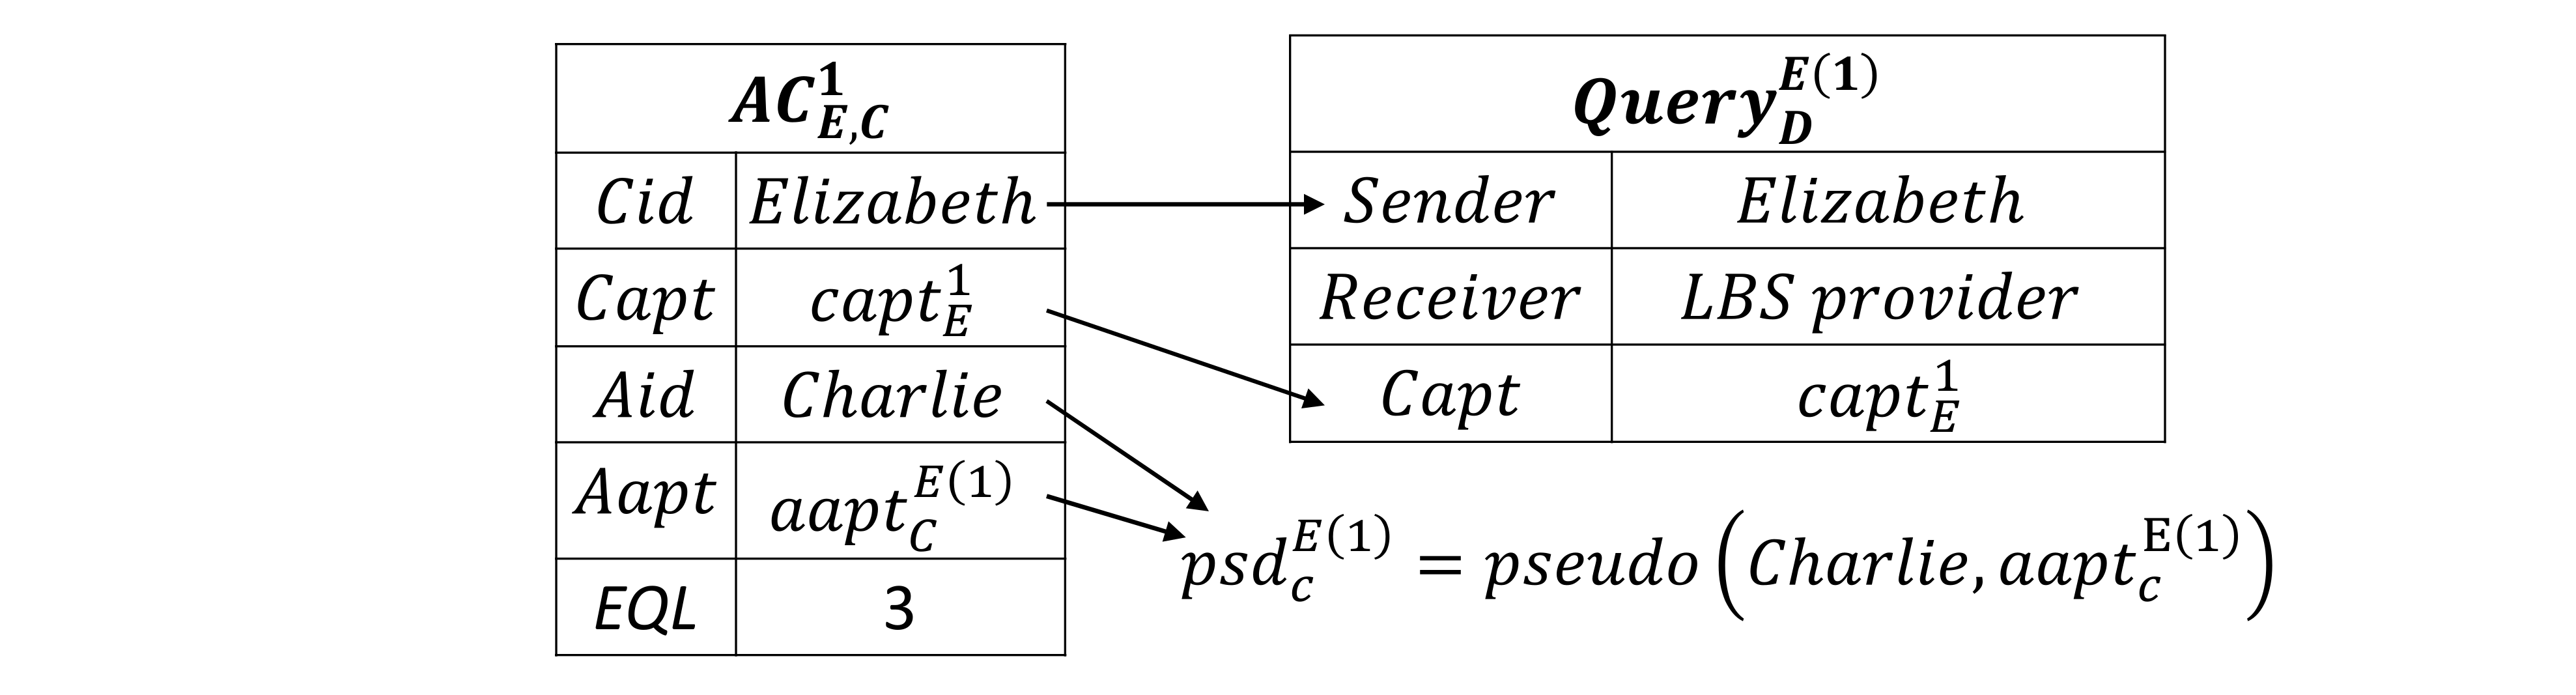
\includegraphics[width=6.0in]{figures/FIG_4_10_Davids_Query.png}
  \caption{David's Query} 
  \label{fig:DavidsQuery} %% label for entire figure 
\end{figure}

The LBS sends a reply message to Elizabeth based on the sender identity of the query. The $Capt$ (i.e., ${capt}^1_E$) is also included in the reply. If an attacker learns these messages, he believes that it is Elizabeth who sends the query.

When Elizabeth receives the reply message, she searches her reply table for the AC used in the reply message, as shown in Table \ref{table:DEReplyTableT8}. Since the message is sent by the LBS, the ${Aid}_{old}$ should equal to her own identity, and the ${Aapt}_{old}$ should equal to the $Capt$. Then she must find an entry like Table \ref{table:ElizabethReplyTableEntry}, which enables Elizabeth to modify the reply message and forward it to Bob, as shown in Figure \ref{fig:ElizabethForwardsAReply}.


\begin{table} [H]
\caption{Elizabeth's Reply Table Entry}
\label{table:ElizabethReplyTableEntry}
\centering
\tabulinesep = 1mm
\begin{tabu}{|c|c|c|c|c|} \hline
${Aid}_{old}$ & ${Aapt}_{old}$ & ${ID}_{nxt}$ & ${Aapt}_{new}$ & \textit{EQL} \\ \hline
$E$ & ${capt}^1_E$ & $B$ & ${aapt}^{E\left(1\right)}_E$ & 1 \\ \hline 
\end{tabu}
\end{table}

\begin{figure} [H]
  \centering 
  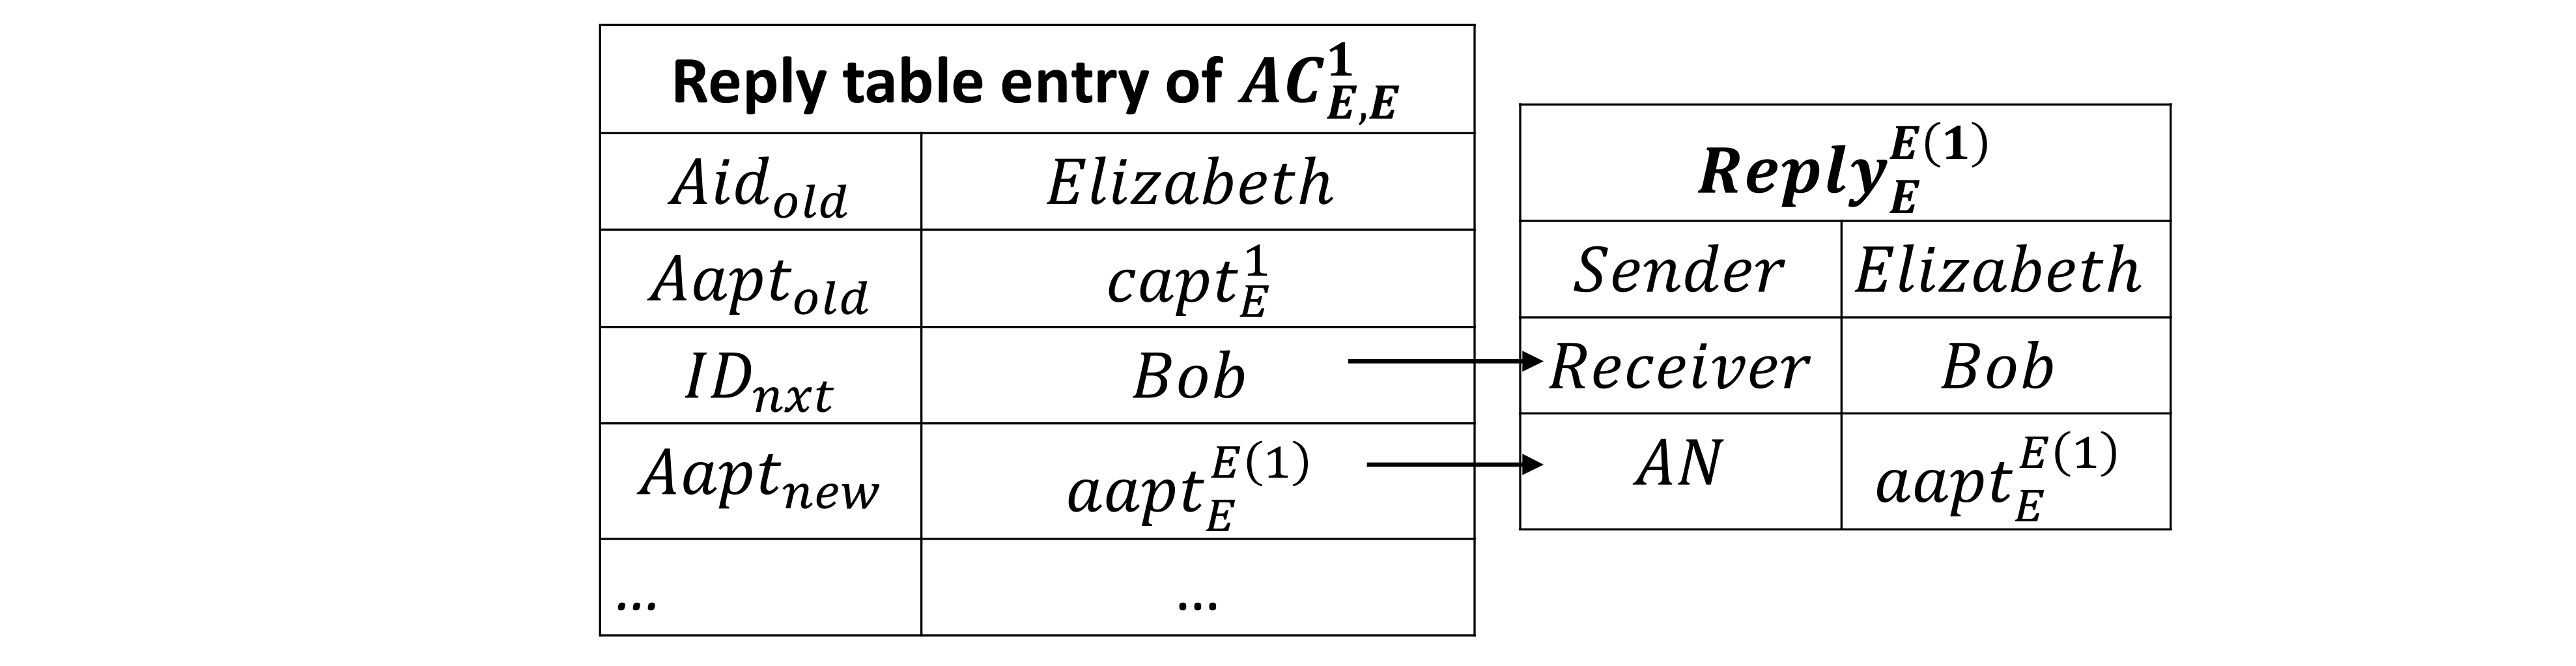
\includegraphics[width=6.0in]{figures/FIG_4_11_Elizabeth_Forwards_A_Reply.png}
  \caption{Elizabeth Forwards A Reply} 
  \label{fig:ElizabethForwardsAReply} %% label for entire figure 
\end{figure}

If Bob receives the reply message successfully, he checks his reply table as shown in Table \ref{table:BCReplyTableT5}. He finds an entry whose ${Aid}_{old}$ is equal to Elizabeth and ${Aapt}_{old}$ is equal to ${aapt}^{E\left(1\right)}_E$, as shown in Table \ref{table:BobsReplyTableEntry}. In the same way as Elizabeth, Bob forwards the reply message to Charlie, as shown in Figure \ref{fig:BobForwardsAReply}.

\begin{table} [H]
\caption{Bob's Reply Table Entry}
\label{table:BobsReplyTableEntry}
\centering
\tabulinesep = 1mm
\begin{tabu}{|c|c|c|c|c|} \hline
${Aid}_{old}$ & ${Aapt}_{old}$ & ${ID}_{nxt}$ & ${Aapt}_{new}$ & \textit{EQL} \\ \hline
$E$ & ${aapt}^{E\left(1\right)}_E$ & $C$ & ${aapt}^{E\left(1\right)}_B$ & 2 \\ \hline 
\end{tabu}
\end{table}

\begin{figure} [H]
  \centering 
  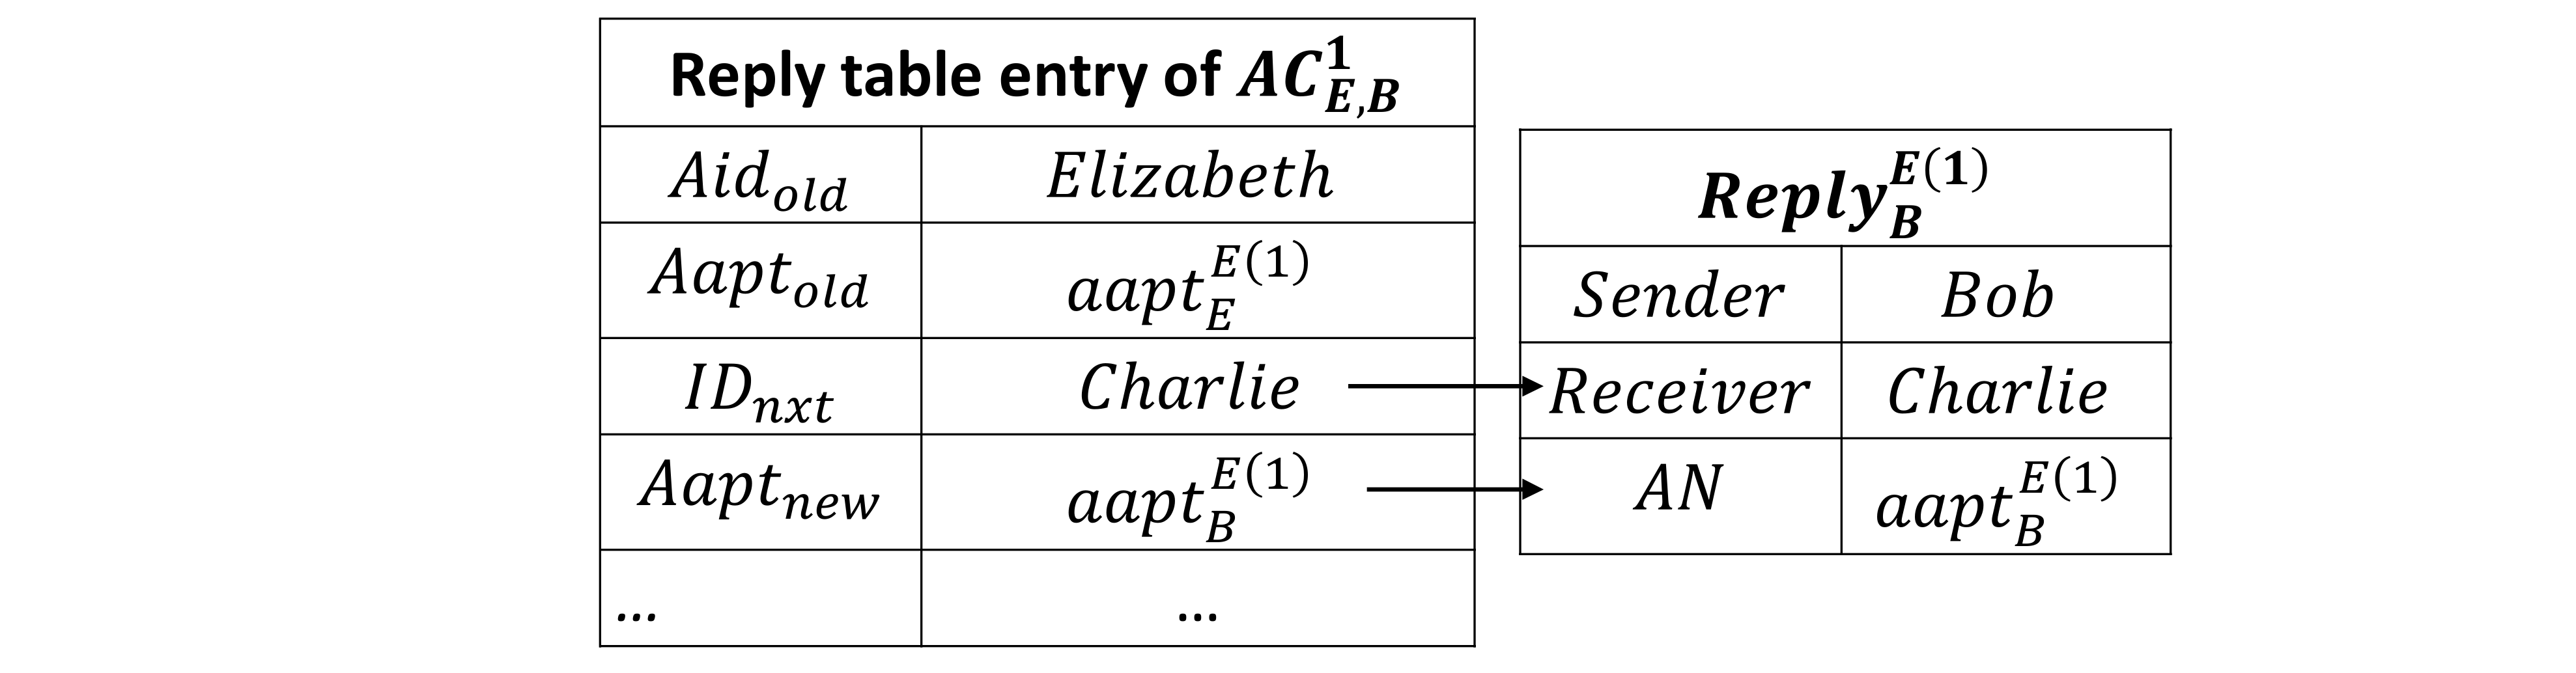
\includegraphics[width=6.0in]{figures/FIG_4_12_Bob_Forwards_A_Reply.png}
  \caption{Bob Forwards A Reply} 
  \label{fig:BobForwardsAReply} %% label for entire figure 
\end{figure}

When the Charlie receives the reply message from Bob, Charlie learns that he is the last agent based on his reply table as shown in Table \ref{table:CDReplyTableT7} and Table \ref{table:CharliesReplyTableEntry}, because the \textit{EQL} is equal to 3. He ignores the record of ${ID}_{nxt}$ $D$ and views it as a $VOID$ because he is the last agent.


\begin{table} [H]
\caption{Charlie's Reply Table Entry}
\label{table:CharliesReplyTableEntry}
\centering
\tabulinesep = 1mm
\begin{tabu}{|c|c|c|c|c|} \hline
${Aid}_{old}$ & ${Aapt}_{old}$ & ${ID}_{nxt}$ & ${Aapt}_{new}$ & \textit{EQL} \\ \hline
$B$ & ${aapt}^{E\left(1\right)}_B$ & $D$($VOID$) & ${aapt}^{E\left(1\right)}_C$ & 3 \\ \hline 
\end{tabu}
\end{table}



To forward the reply message to the unknown original requester (i.e., David), Charlie generates a pseudonym ${psd}^{E\left(1\right)}_c=\mathrm{pseudo}\left(Charlie,{aapt}^{\mathrm{E}\left(1\right)}_c\right)$ using his own identity and ${Aapt}_{new}$. We should notice that the pseudonym is exactly the temporary identity of David. David then modifies the reply message and forwards it, as shown in Figure \ref{fig:CharlieForwardsAReply}.

\begin{figure} [H]
  \centering 
  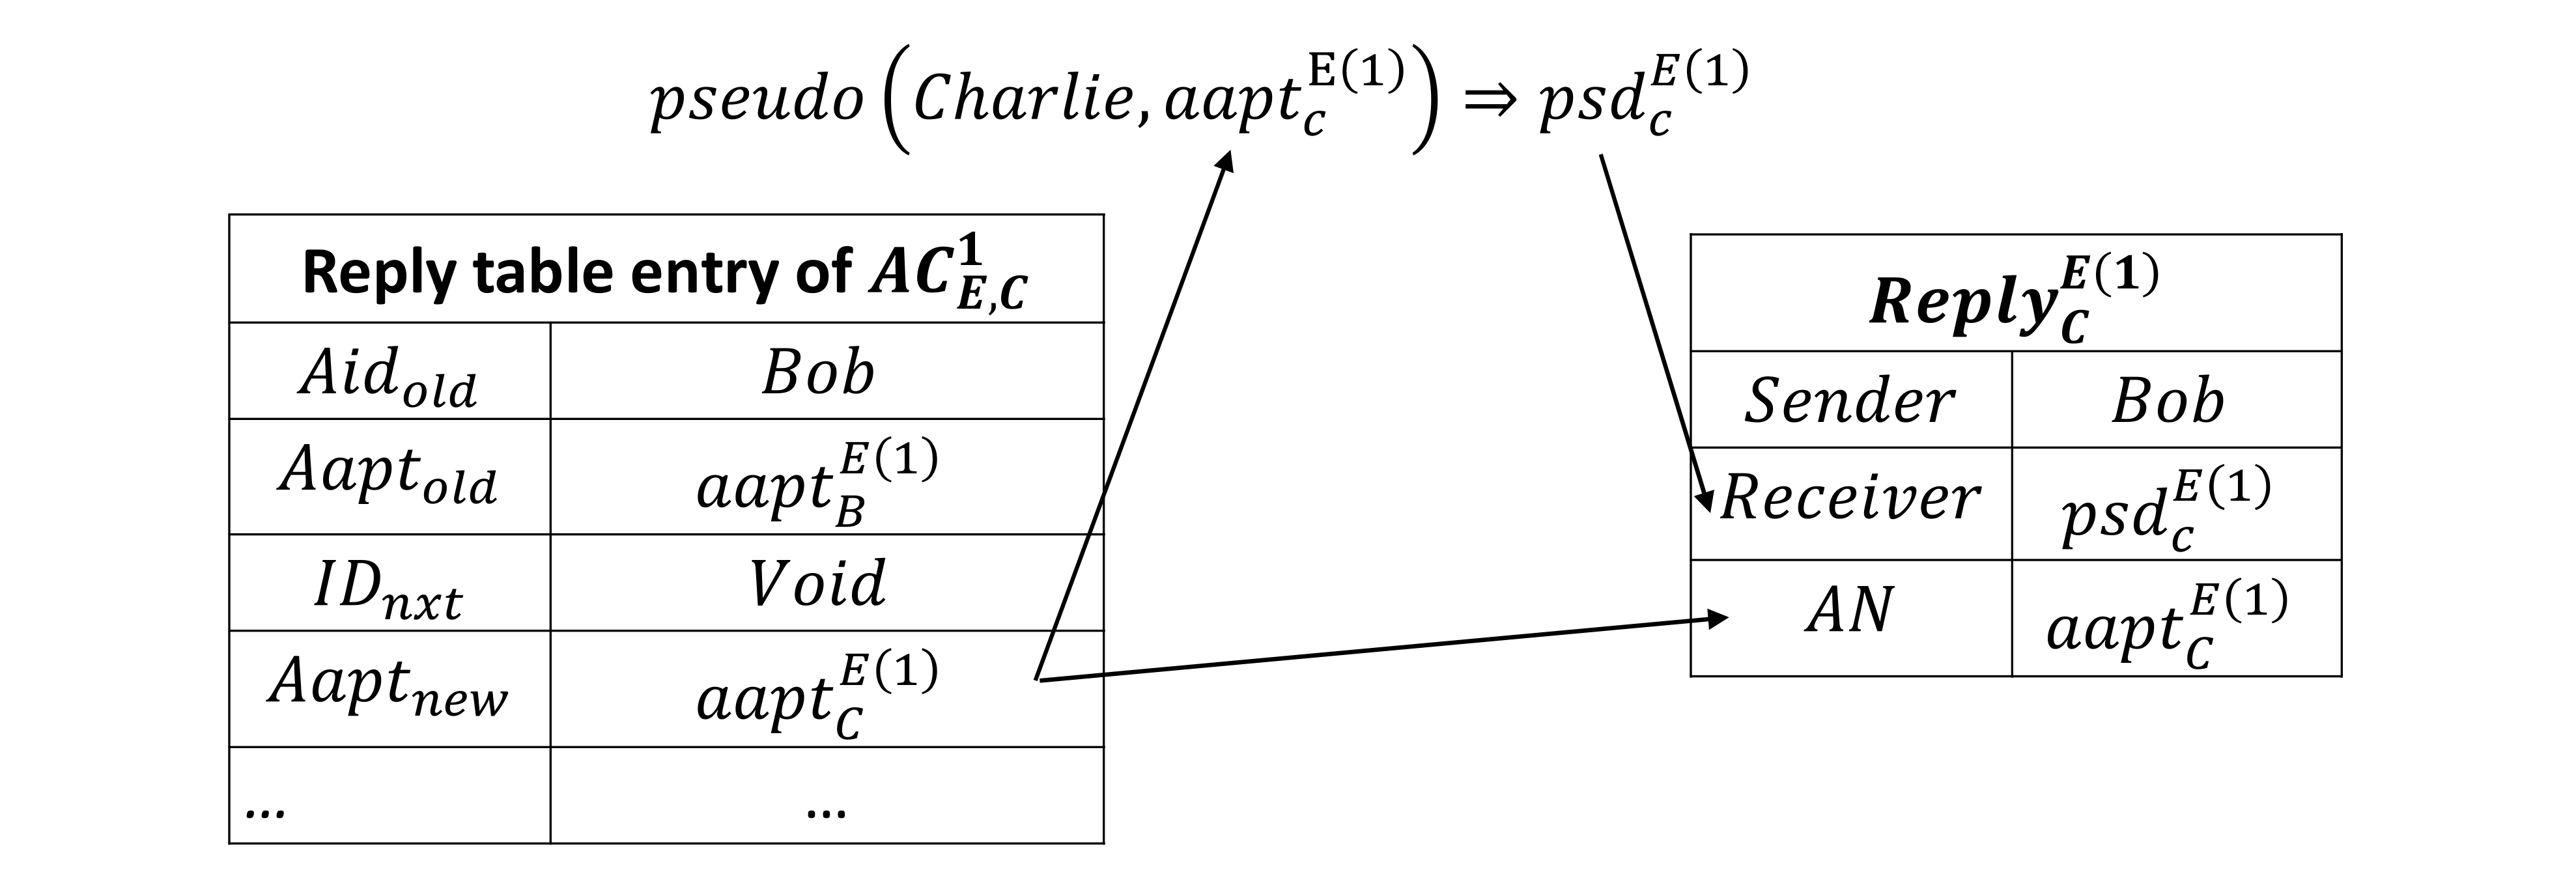
\includegraphics[width=6.0in]{figures/FIG_4_13_Charlie_Forwards_A_Reply.png}
  \caption{Charlie Forwards A Reply} 
  \label{fig:CharlieForwardsAReply} %% label for entire figure 
\end{figure}

When a user who carries ${Reply}^{E\left(1\right)}_C$ encounters David, the user forwards the reply to him, so that David gets his reply.

